\documentclass[12pt]{beamer}
\usepackage{beamerthemeHannover, graphicx, clrscode, amsmath, amssymb, multicol}
\usepackage{textcomp}
\usepackage{verbatim}
\setbeamercolor{sidebar}{use=structure,bg=gray!60!green}

\title{PL/Parrot and PL/Perl6 \\ \small {Parrots and Butterflies in your Database} }
\author[@dukeleto]{Jonathan "Duke" Leto}
\date{}

\begin{document}

\frame{
    \titlepage
    \begin{center}
    \end{center}
}

\frame{
    \frametitle{Parrot Virtual Machine}
    \begin{center}
        \begin{itemize}
            \item Process (Application) Virtual Machine
            \item Register-based
            \item Continuation Passing Style
            \item Design Goals
            \begin{itemize}
                \item Pluggable
                \item Interoperable
                \item Dynamic
            \end{itemize}
        \end{itemize}
    \end{center}
}
\frame{
    \frametitle{Rakudo Perl 6}
    \begin{center}
        \begin{itemize}
            \item Most active implementation of Perl 6
            \item Implements $\sim 80\%$ of the spec
            \item Currently uses Parrot as a backend, but plans to support others
            \item Stable release series is Rakudo Star, dev release every month
        \end{itemize}
    \end{center}
}

\frame{
    \frametitle{Why Embed Parrot VM in PostgreSQL?}
    \begin{center}
        \begin{itemize}
            \item PL's are (very) hard to write and maintain
            \item Framework for DSL's
            \item Platform independent, fast, stored procedures
            \item Allow various PL's to communicate
            \item Freeze/thaw subtransaction-level states
        \end{itemize}
    \end{center}
}

\frame{
    \frametitle{History of PL/Parrot}
}

\frame{
    \frametitle{Current Features}
    \begin{itemize}
        \item PL/PIR and PL/Perl6
        \item Pass and return basic datatypes
        \item Basic security model (Don't do that)
        \item Growing Test Suite
        \item Enthusiastic and friendly community
        \item Coolest Feature: Use Perl 6 grammars in PostgreSQL!
    \end{itemize}
}

\frame{
    \frametitle{Bugs}
    \begin{itemize}
        \item Documentation
        \item SPI
        \item Triggers
        \item Parrot Bugs
        \begin{itemize}
            \item IMCC Syntax Errors
            \item Security API
        \end{itemize}
    \end{itemize}
}

\frame{
    \frametitle{PL/PIR Example 1}
    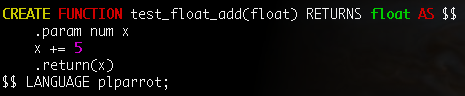
\includegraphics[width=9.5cm, height=3.6cm]{plparrot_example_code}
}

\frame{
    \frametitle{Installing PL/Parrot: Method 1}
    \begin{itemize}
        \item Install Rakudo or Parrot
        \item \# parrot\_config needs to be in your \textdollaroldstyle PATH
        \item One of:
        \item git clone git://github.com/leto/plparrot.git
        \item wget http://icanhaz.com/plparrot0.20
        \item cd plparrot
        \item export PGPORT=5555 \# if necessary
        \item make install installcheck \# might need sudo
        \item make test\_plperl6 \# Run PL/Perl6 tests
    \end{itemize}
}

\frame{
    \frametitle{Future Goals}
    \begin{itemize}
        \item Tools to help easily create a new DSL with PL/Parrot
        \item Easy onramps to add new languages to PL/Parrot
    \end{itemize}
}

\frame{
    \frametitle{Get involved!}
    \begin{itemize}
        \item Try PL/Parrot on your system and submit detailed bug reports
        \item Fork on github and hack on stuff!
        \item Help with GitHub Issues
        \item \#plparrot on freenode
        \item http://pl.parrot.org
        \item http://groups.google.com/group/plparrot
    \end{itemize}
}

\frame{
    \frametitle{ Thanks }
    \begin{itemize}
        \item PL/Parrot team:
            \begin{itemize}
            \item David Fetter, David E. Wheeler, Joshua Tolley, Daniel Arbelo Arrocha, Dave Olszewski
            \item AKA davidfetter++, theory++, eggyknap++, darbelo++, cxreg++
            \end{itemize}
        \item Everyone working on Parrot Virtual Machine, Perl 6 and PostgreSQL
        \item Especially (Moritz Lenz) moritz++, (Peter Lobsinger) plobsing++ and (Stephen O'Rear) sorear++, for great advice and help
    \end{itemize}
}

\frame{
    \frametitle{ Resources }
    \begin{center}
        \begin{itemize}
           \item http://pl.parrot.org
           \item http://github.com/leto/plparrot
           \item http://parrot.org
           \item @parrotvm / !parrot on twitter/identi.ca
           \item @dukeleto / @leto on twitter/identi.ca
        \end{itemize}
    \end{center}
}
\end{document}
